\pagestyle{fancy}
\fancyhead[LE,RO]{\thepage}
\fancyhead[RE]{Apéndice} %
\fancyhead[LO]{\nouppercase{\rightmark}}
%\fancyhead[RE]{Parte \thepart \rightmark} %

\chapterbegin{Cable serie y bootloaders}
\label{chp:SerieBoot}
\minitoc

\section{Introducción}

En esta sección profundizamos sobre dos métodos para cargar programas en Bare Metal sin
necesidad de insertar y extraer continuamente la tarjeta SD. Existe un tercer método que
no explicamos aquí, el del cable JTAG, pero pueden consultar los archivos
README del repositorio de David Welch\cite{DWEL}.

Este apéndice está basado en el contenido de dicho repositorio, y el código fuente del
bootloader que mostramos aquí es idéntico, el cual reproducimos con permiso del autor.

\section{Cable USB-serie desde el ordenador de desarrollo}

Con esta opción hacemos todo el trabajo de ensamblado y enlazado en nuestro ordenador
de desarrollo, para luego transferir el archivo Bare Metal por el puerto serie
directamente a la Raspberry. Necesitamos un adaptador USB-serie como el de la siguiente
figura \ref{fig:mapamemoria}.

\begin{figure}[h]
  \centering
    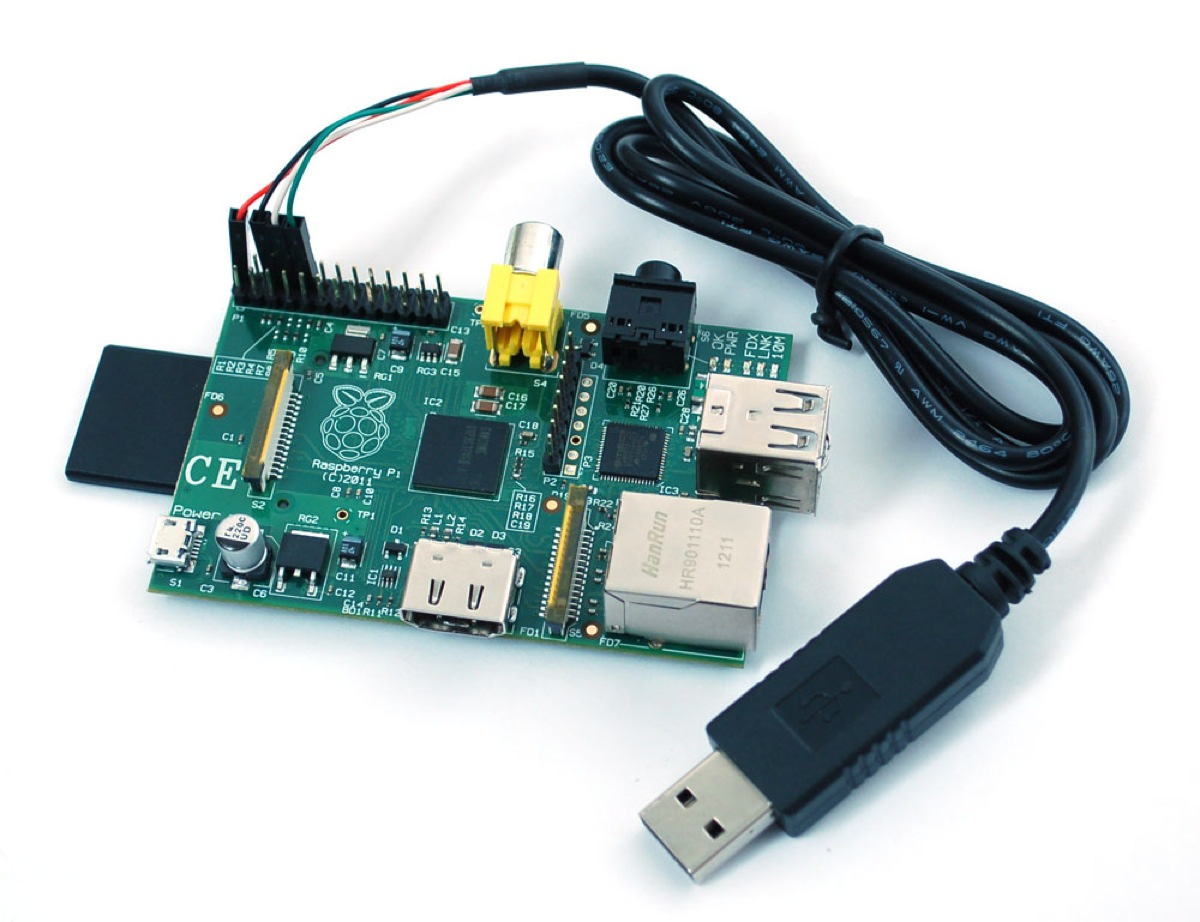
\includegraphics[width=14cm]{graphs/ARM_RaspberryPi_serial.jpg}
  \caption{Cable USB-serie}
  \label{fig:cableusb}
\end{figure}

Lo primero que tenemos que hacer es cargar el bootloader
\footnote{\url{https://github.com/dwelch67/raspberrypi/blob/master/bootloader05/kernel.img?raw=true}}
en la SD y alimentar la Raspberry. Es necesario resetear la Raspberry cada vez que
queramos cargar un programa Bare Metal nuevo, y esto se hace manualmente desenchufando y
enchufando la alimentación, o bien con el método automático que explicamos en la última sección.

Debemos conectar los 3 cables que van del adaptador USB-serie a la Raspberry, con los pines
tercero, cuarto y quinto de la fila superior del puerto GPIO. El tercer pin es la masa, en el
adaptador es un cable negro o marcado con GND en la serigrafía. El cuarto pin es GPIO 14 ó TXD,
que se corresponde con el pin RXD en el adaptador. Por último el quinto pin es GPIO 15 ó RXD y
va conectado al pin TXD del adaptador. Nótese que los cables están cruzados, el pin que
transmite desde el PC es el que recibe en la Raspberry y viceversa.

La primera vez que probemos el cable es recomendable probar con un programa simple como un
LED parpadeante, por ejemplo el último {\tt esbn5.s} del capítulo \ref{chp:Subrut}. A partir
del código fuente generamos el binario en Bare Metal, para lo cual necesitamos el toolchain
(cadena de herramientas) ARM, de la que usaremos el ensamblador {\tt as}, el enlazador {\tt ld}
y el copiador de secciones {\tt objcopy}. A estas herramientas, que generan binarios
o ejecutables para una plataforma diferente a la de la máquina que realiza la compilación,
se las denomina {\it herramientas de compilación cruzada}.

En estos momentos tenemos el binario Bare Metal generado, llamémoslo {\tt esbn5.img}. El
siguiente paso es enviar este archivo por el puerto serie de forma que se ejecute en la
Raspberry. Pero no lo enviamos de cualquier manera, sino que emplearemos un protocolo
de transferencia que se llama XMODEM. Por suerte es uno de los protocolos mejor soportados
por los emuladores de terminal.

Dependiendo de nuestra plataforma hay distintos emuladores de terminal disponibles. Para
Windows tenemos {\tt HyperTerminal} o {\tt Tera Term}, y en Linux tenemos {\tt minicom},
aunque para lo que queremos hacer (enviar un archivo) nos basta con el comando {\tt sx}.

Antes de nada hay que configurar los parámetros del puerto serie en el emulador de
terminal que estemos empleando. Los valores son: 8 bits de datos, sin paridad, 1 bit de
parada, sin flujo de control y velocidad de transferencia de 115200 baudios. Son todos
parámetros por defecto excepto la velocidad, por lo que hay que asegurarse de cambiar
la velocidad antes de proceder a transferir el archivo.

Luego elegimos el protocolo, {\tt XMODEM}, y le damos a transferir, seleccionando
nuestro {\tt esbn5.img} como archivo de origen. Si todo ha ido bien debería aparecer
un mensaje indicándolo en nuestro programa terminal y observaremos el LED parpadenado
en la Raspberry, prueba de que la transferencia ha sido exitosa.

En Linux es fácil automatizar este proceso con el comando {\tt sx}, que es creando
el siguiente script {\tt enviar}.

\begin{lstlisting}
stty -F /dev/ttyUSB0 115200
sx $1 < /dev/ttyUSB0 > /dev/ttyUSB0
\end{lstlisting}

Y para enviar el archivo anterior con este script escribimos bajo línea de comandos lo siguiente.

\begin{lstlisting}
./enviar esbn5.img
\end{lstlisting}

\section{Cable serie-serie que comunica dos Raspberries}

Esta configuración es ideal si queremos emplear una Raspberry como ordenador de desarrollo.
Aunque también está la alternativa de trabajar con un ordenador de desarrollo aparte conectado
a una de las Raspberries mediante {\tt ssh}. La ventaja de esta última alternativa es que podemos
compilar desde la Raspberry sin necesidad de tener instaladas las herramientas de compilación
cruzada en tu ordenador. Y otra ventaja es que no necesitas estar físicamente cerca de la
Raspberry ni tener enchufado el adaptador USB, te puedes conectar inalámbricamente a la Raspberry
mediante un router Wifi (con cable Ethernet entre el router y la Raspberry).

Lo primero es diferenciar las dos Raspberries. A una la llamamos Raspberry de desarrollo,
en la cual tendremos instalado Raspbian y es en la que trabajamos directamente (con teclado y
pantalla) o bien nos conectamos con ella mediante ssh. A la otra la llamamos Raspberry Bare
Metal, en la que sobreescribimos el kernel.img de la SD con el mismo bootloader de antes. Es
en esta Raspberry donde se ejecutan los programas Bare Metal que vamos a desarrollar y por tanto
donde enchufaremos nuestra placa auxiliar.

La conexión entre ambas Raspberries se hace uniendo ambas masas y cruzando los cables TXD
y RXD de cada puerto serie, como viene indicado en la figura \ref{fig:pitopi}.

\begin{figure}[h]
  \centering
    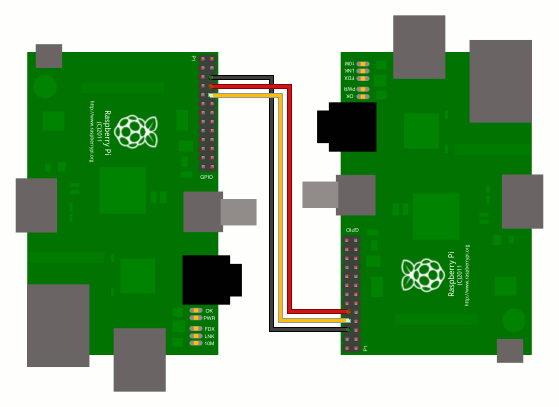
\includegraphics[width=14cm]{graphs/pitopi.png}
  \caption{Dos raspberries en serie cruzado}
  \label{fig:pitopi}
\end{figure}

Por defecto el puerto serie en Raspbian viene configurado como salida de consola. Esta
configuración no nos interesa, se usa para diagnosticar errores mostrando por un terminal
los mensajes del arranque. Pero nosotros queremos usarlo como un puerto serie genérico,
para lo cual es necesario hacer los siguientes cambios.

En el archivo {\tt /etc/inittab} descomentamos la línea que empieza con {\tt T0:23...} y
que hace mención a la cadena {\tt ttyAMA0}, y guardamos el archivo.

Luego en el archivo {\tt /boot/cmdline.txt} buscamos los dos sitios (puede haber uno sólo)
donde aparece {\tt ttyAMA0}. Borramos los textos que hay entre espacios y que incluyen el
{\tt ttyAMA0}, y después guardamos.

Para comprobar que todo ha ido bien reseteamos la Rasbperry con {\tt sudo reboot} y tras
el arranque escribimos.

\begin{lstlisting}
cat /proc/cmdline
\end{lstlisting}

Comprobando que efectivamente no hay se hace ninguna referencia a {\tt ttyAMA0}, y luego
escribimos este otro comando.

\begin{lstlisting}
ps aux | grep ttyAMA0
\end{lstlisting}

Para verificar que el único proceso que se lista en la salida es el del propio comando {\tt ps}
y no existen otros.

Llegados a este punto ya tenemos el puerto serie disponible para nosotros. El resto de pasos
serían como en el caso anterior, pero cambiando la referencia que se hace al puerto. Donde
antes aparecía {\tt /dev/ttyUSB0} (o algo similar) lo cambiamos por {\tt /dev/ttyAMA0}.

\section{Reseteo automático}

Resulta tedioso tener que desenchufar y enchufar la Raspberry cada vez que queremos introducir
un nuevo programa Bare Metal. Una solución intermedia es soldar los dos pines de Reset que
están serigrafiados como {\tt P6} en la Raspberry 2.0 o como {\tt RUN} en el modelo A+/B+.
A éstos pines le podemos conectar un pulsador, con simplificamos el reseteo, en lugar de
desenchufar y enchufar pulsamos un botón.

Sin embargo es muy conveniente buscar una solución totalmente automática, mediante la cual
el propio script que envía el archivo envíe una señal de Reset justo antes del envío. Para
evitar confusiones, en lugar de montar los dos pines del conector, montamos sólo uno, el
de la señal que provoca el Reset (el otro es la masa). Viene señalada con un círculo rojo
en la figura \ref{fig:pinReset}.

\begin{figure}[h]
  \centering
    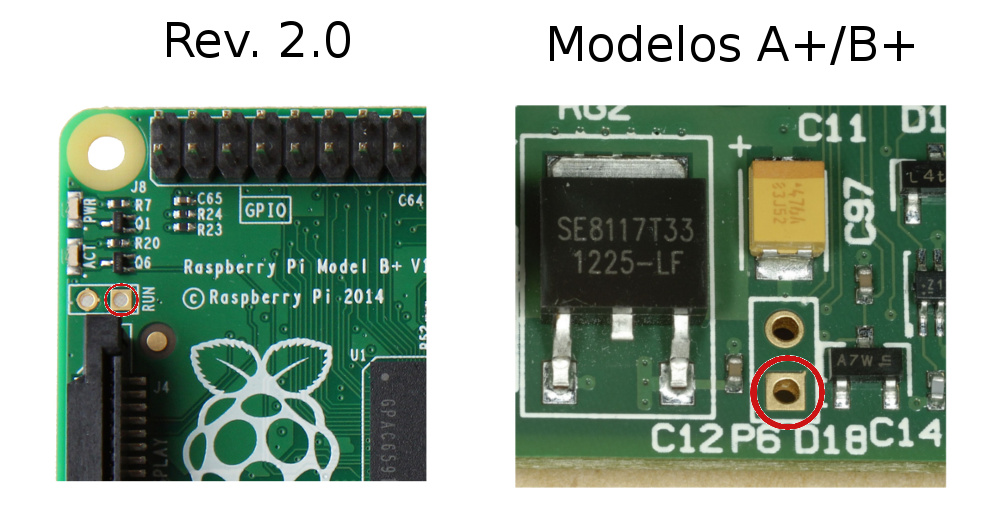
\includegraphics[width=14cm]{graphs/pinReset.jpg}
  \caption{Señal de Reset donde montar el pin}
  \label{fig:pinReset}
\end{figure}

De lo que se trata ahora es de enviar un pulso negativo a esa señal. En el caso del cable
USB-Serie lo haremos por una señal programable que no se emplea en el enlace serie llamada
{\tt DTR}. En el caso de conexión serie-serie entre dos Raspberries usaremos el pin GPIO 18
(justo a la derecha de RXD), valdría cualquier otro pin, pero por cercanía empleamos este.

Lo siguiente es hacer un programa que envíe dicho pulso en incluirlo en el script. Para
el cable USB-Serie empleamos este programa.

\begin{lstlisting}
int pulseDTR(int fd){
    int status;

    // leemos la señal de control status
    if (ioctl(fd, TIOCMGET, &status) == -1) {
        // manejamos el error
    }

    // Ponemos DTR a cero (activamos reset)
    status &= ~TIOCM_DTR;
    // y lo aplicamos a la señal de control
    if (ioctl(fd, TIOCMSET, &status) == -1) {
        // manejamos el error
    }
    // esperamos un poco
    usleep (400*1000);
    // Ahora ponemos DTR a uno (desactivamos reset)
    status |= TIOCM_DTR;
    // y lo aplicamos
    if (ioctl(fd, TIOCMSET, &status) == -1) {
        // manejamos el error
    }
    return 0;
}
\end{lstlisting}

En el caso de las dos Raspberries instalamos primero el paquete {\tt wiringPi}.

\begin{lstlisting}
git clone git://git.drogon.net/wiringPi
cd wiringPi
./build
\end{lstlisting}

E incluímos el pulso reset mediante comandos, por ejemplo nuestro script que compila
y envía el archivo (todo en un paso) quedaría así.

\begin{lstlisting}
gpio export 18 out
as -o tmp.o $1
gpio export 18 in
ld -e 0 -Ttext=0x8000 -o tmp.elf tmp.o
objcopy tmp.elf -O binary tmp.img
stty -F /dev/ttyAMA0 115200
sx tmp.img < /dev/ttyAMA0 > /dev/ttyAMA0
\end{lstlisting}

Observamos que el pulso de reset dura lo que tarde el programa en ensamblar, duración
más que suficiente como para provocar un Reset en la Raspberry Bare Metal. Para llamar
al script escribimos algo como esto.

\begin{lstlisting}
./compila esbn5.s
\end{lstlisting}

\section{Código fuente del bootloader}

Mostramos la parte principal del programa bootloader, el resto de archivos están
en el repositorio.

\begin{lstlisting}[caption={bootloader05.c},label={lst:bootloader}]
//-----------------------------------
unsigned char xstring[256];
//-----------------------------------
int notmain ( void )
{
    unsigned int ra;
    unsigned int rx;
    unsigned int addr;
    unsigned int block;
    unsigned int state;

    unsigned int crc;

    uart_init();
    hexstring(0x12345678);
    hexstring(GETPC());
    hexstring(ARMBASE);
    timer_init();

//SOH 0x01
//ACK 0x06
//NAK 0x15
//EOT 0x04

//block numbers start with 1

//132 byte packet
//starts with SOH
//block number byte
//255-block number
//128 bytes of data
//checksum byte (whole packet)
//a single EOT instead of SOH when done, send an ACK on it too

    block=1;
    addr=ARMBASE;
    state=0;
    crc=0;
    rx=timer_tick();
    while(1)
    {
        ra=timer_tick();
        if((ra-rx)>=4000000)
        {
            uart_send(0x15);
            rx+=4000000;
        }
        if((uart_lcr()&0x01)==0) continue;
        xstring[state]=uart_recv();
        rx=timer_tick();
        if(state==0)
        {
            if(xstring[state]==0x04)
            {
                uart_send(0x06);
                for(ra=0;ra<30;ra++) hexstring(ra);
                hexstring(0x11111111);
                hexstring(0x22222222);
                hexstring(0x33333333);
                uart_flush();
                BRANCHTO(ARMBASE);
                break;
            }
        }
        switch(state)
        {
            case 0:
            {
                if(xstring[state]==0x01)
                {
                    crc=xstring[state];
                    state++;
                }
                else
                {
                    //state=0;
                    uart_send(0x15);
                }
                break;
            }
            case 1:
            {
                if(xstring[state]==block)
                {
                    crc+=xstring[state];
                    state++;
                }
                else
                {
                    state=0;
                    uart_send(0x15);
                }
                break;
            }
            case 2:
            {
                if(xstring[state]==(0xFF-xstring[state-1]))
                {
                    crc+=xstring[state];
                    state++;
                }
                else
                {
                    uart_send(0x15);
                    state=0;
                }
                break;
            }
            case 131:
            {
                crc&=0xFF;
                if(xstring[state]==crc)
                {
                    for(ra=0;ra<128;ra++)
                    {
                        PUT8(addr++,xstring[ra+3]);
                    }
                    uart_send(0x06);
                    block=(block+1)&0xFF;
                }
                else
                {
                    uart_send(0x15);
                }
                state=0;
                break;
            }
            default:
            {
                crc+=xstring[state];
                state++;
                break;
            }
        }
    }
    return(0);
}
\end{lstlisting}

Al comienzo se envían tres cadenas en hexadecimal por el puerto (0x12345678, GETPC() y ARMBASE)
para indicar que el bootloader está listo para recibir. Esto lo podemos ver si empleamos un
programa terminal como {\tt minicom} para leer del puerto.

Después se inicializan algunas variables y nos metemos en el bucle principal. Se supone que el
primer byte que tenemos que recibir desde el host es {\tt SOH}, en hexadecimal es {\tt 0x01}.
Si pasado un tiempo no recibimos nada, enviamos un {\tt NAK} ({\tt 0x15}) para indicarle al host
que estamos vivos. En realidad este comando sirve para decirle al host que el paquete recibido
es erróneo, que nos lo envíe nuevamente.

El host enviará a la Raspberry el archivo en trozos de 128 bytes cada uno (rellenando el último
trozo con ceros hasta que ocupe 128 bytes) con este formato.

\begin{figure}[h]
  \centering
    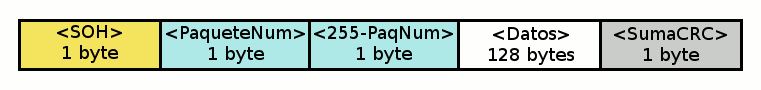
\includegraphics[width=14cm]{graphs/xmodem.png}
  \caption{Formato de paquete XMODEM}
  \label{fig:xmodem}
\end{figure}

Se trata del byte {\tt SOH} seguido del número de bloque, luego tenemos otra vez el número de
bloque pero complementado, a continuación los 128 bytes de datos para acabar con un último byte
de suma de comprobación. Este último byte es la suma de todos los anteriores, quedándonos con
los 8 bits menos significativos del resultado.

Entonces la Raspberry lleva la cuenta del byte por el que vamos dentro de dicho paquete a
partir de {\tt switch(state)}. De tal forma que si {\tt state} vale 0, lo que esperamos es
{\tt SOH} o {\tt EOT}, cualquier otro valor indica que algo va mal por tanto enviamos un
{\tt NAK} al host y ponemos {\tt state} a cero.

Para los estados 1 y 2 simplemente comprobamos que el byte recibido coincide con el número
de bloque, y reportamos error en caso contrario de la misma forma que antes (enviando
{\tt NAK} y {\tt state=0}).

Luego tenemos los estados que van entre 3 y 131, en los que vamos escribiendo el fichero en
memoria e incrementando el puntero, a la vez que vamos calculando el byte de suma para
la comprobación.

Por último tenemos el estado 131, en el cual ya hemos recibido los bytes de datos y lo que
leemos ahora es el byte de suma de comprobación. Comparamos que coincide con el valor esperado,
respondiendo con {\tt ACK}, o notificamos del error como siempre (con {\tt NAK} y {\tt state=0}).

En cuanto el host recibe el {\tt ACK} del último paquete enviado, éste en lugar de enviar
de nuevo un paquete completo, envía un sólo byte, {\tt EOT}, para indicar a la Raspberry
que ya no quedan más paquetes por enviar y se acaba la transmisión.

Esta situación la comprueba la Raspberry al principio de cada paquete, de tal forma que si
recimibos un {\tt EOT} del host damos por acabada la transmisión y ejecutamos el archivo
Bare Metal leído con {\tt BRANCHTO}, que en bajo nivel se corresponde con saltar a {\tt 0x8000}.

En la figura \ref{fig:transm} tenemos un ejemplo completo de transmisión. En él se envían 4
paquetes, con errores y reenvíos en los paquetes 2 y 3. Podría tratarse de un archivo que
ocupase 500 bytes, y que la utilidad {\tt sx} haya rellenado en el último paquete 12 bytes
con ceros, para que de esta forma todos los paquetes ocupen 128 bytes (la parte útil, contando
cabeceras y demás cada paquete ocupa 132 bytes).

\begin{figure}[h]
  \centering
    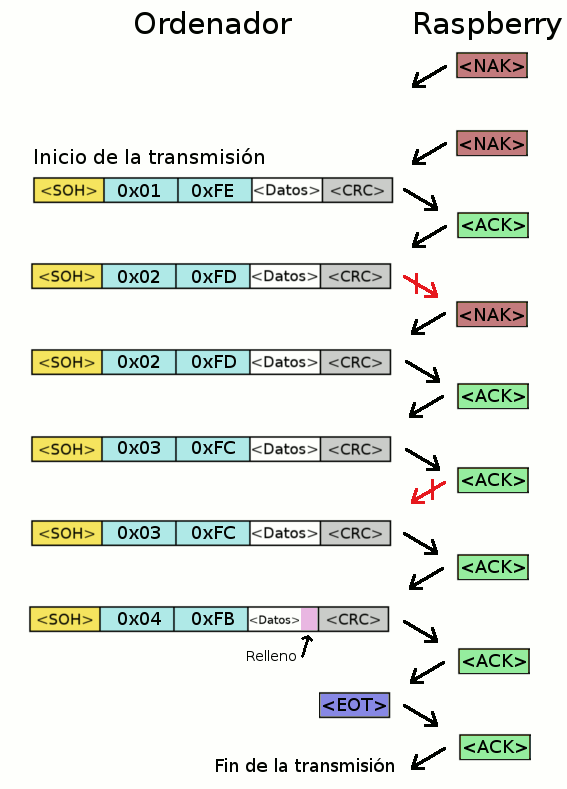
\includegraphics[width=14cm]{graphs/transm.png}
  \caption{Ejemplo de transmisión}
  \label{fig:transm}
\end{figure}

\chapterend
